\documentclass[12pt]{beamer}
\usepackage[utf8]{vietnam}
\usepackage{lmodern}
\usepackage{animate}
\usepackage{wrapfig}
\usetheme{metropolis}

\begin{document}
	\author{Đặng Quang Anh - Cao Việt Tùng}
	\title{TABU SEARCH}
	\date{Tháng 6 2021}
	%\subtitle{}
	%\logo{}
	%\institute{}
	%\date{}
	%\subject{}
	%\setbeamercovered{transparent}
	%\setbeamertemplate{navigation symbols}{}
	\maketitle
	
	\frame<beamer>{
		\frametitle{Outline}
		\tableofcontents
	}
	
	\section{Search Space and Neighbor Structure}
	\begin{frame}
		\frametitle{Search Space and Neighbor Structure}
		\begin{itemize}
			\item Không gian tìm kiếm: Là khoảng không gian của tất cả các giải pháp có thể xem xét (ghé thăm) trong quá trình tìm kiếm.
			\item Cấu trúc vùng lân cận: Là một tập con của Không gian tìm kiếm định nghĩa bởi\\
			$N(S) = \{ $giải pháp thu được bằng cách áp dụng một biến đổi cục bộ duy nhất cho S$ \}$
		\end{itemize}
	\end{frame}
	
	\begin{frame}
		\frametitle{Search Space and Neighbor Structure}
		Ví dụ:\\
		Một người giao hàng cần đi giao hàng tại 5 thành phố. Xuất~phát từ một thành phố bất kì, đi qua các thành phố khác  và trở về thành phố ban đầu, mỗi thành phố chỉ đến một lần. Hãy tìm một đường đi thỏa mãn điều kiện trên sao cho tổng độ dài đường đi là nhỏ nhất.\\
		\begin{itemize}
			\item Không gian tìm kiếm là tập hợp tất cả các cách đi khả~thi của người bán hàng
			\item Với một cách đi S của người bán hàng (giả sử là a-b-c-d-e) thì bằng cách đổi chỗ 2 thành phố bất kì trong cách đi trên ta thu được một cách đi (ví dụ a-c-b-d-e) và đó là một lân cận của S.
		\end{itemize}
	\end{frame}
	
	\section{Tabus}
	\begin{frame}
		\frametitle{Giải thuật leo đồi (Hill Climbing)}
		Giải thuật leo đồi: Ở mỗi lần lặp, tìm giải pháp tốt hơn giải pháp hiện tại trong vùng lân cận, nếu không có thì thuật toán dừng lại. Điều đó dẫn đến thuật toán có thể bị kẹt lại tối ưu cục bộ.\\
		Ví dụ:\\
		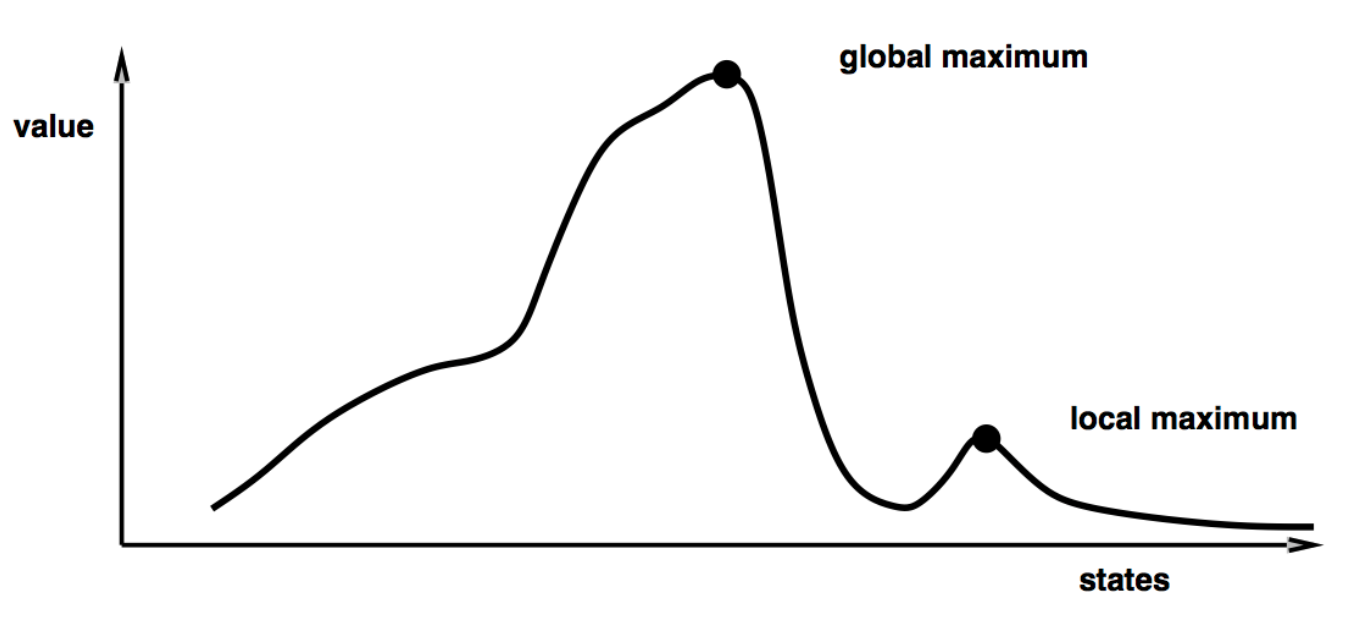
\includegraphics[scale=0.4]{HillClimbing.png}\\
	\end{frame}
	
	\begin{frame}
		\frametitle{Tabus}
		Tabu Search cho phép di chuyển khỏi tối ưu cục bộ bằng các bước đi không cải thiện hàm mục tiêu.\\
		Khi đó, có khả năng rằng thuật toán sẽ đi ngược lại những bước đã đi qua và trở về điểm xuất phát. Như vậy ta cần làm gì đó để ngăn không cho điều này xảy ra.\\
		Ta thực hiện việc này bằng cách sử dụng Tabus.
	\end{frame}
	
	\begin{frame}
		\frametitle{Tabus}
		%		Một bước đi được gọi là Tabu nếu nó đã được đi trong một số lần tìm kiếm trước đó.\\
		Tabus được lưu trữ trong bộ nhớ ngắn hạn của cuộc tìm kiếm (tabu list)\\
		Ví dụ:\\
		Như ở ví dụ trước từ a-b-c-d-e ta đã đổi chỗ b từ vị trí 2 đến 3 để có a-c-b-d-e nên tabus có thể lưu $(b, 3, 2)$ nghĩa là ngăn b di chuyển từ 3 về 2 hoặc $(b, 2)$ để ngăn b di chuyển về 2 bất kể đang ở đâu hay đơn giản là $(b)$ để ngăn không cho b di chuyển.
	\end{frame}
	
	\section{Aspiration Criterion}
	\begin{frame}
		\frametitle{Aspiration Criterion}
		Ví dụ:\\
		Maximum: $f(x) = -x^{12} + 3x^3 - x$
		\begin{wrapfigure}{r}{5cm}
			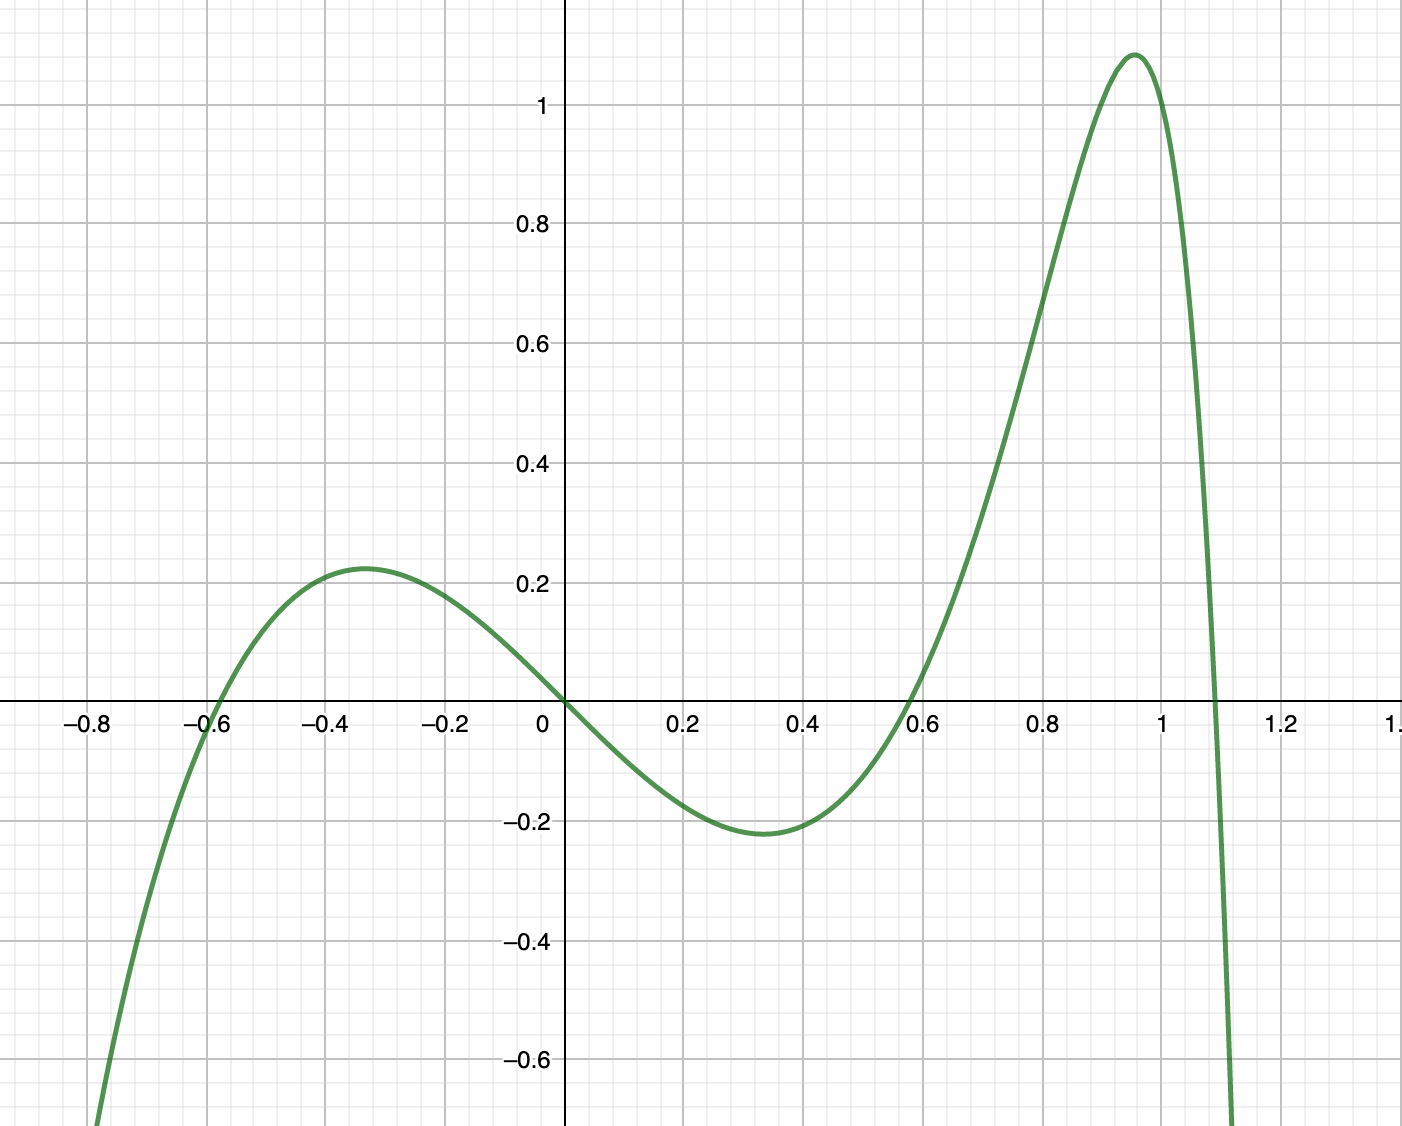
\includegraphics[width=4.5cm]{AC.png}
		\end{wrapfigure}
		Với $x$ từ $-\infty$ đến $+\infty$ ta thấy rằng nếu sử dụng thuật toán leo đồi thì sẽ chỉ trả về kết quả là cực đại địa phương nhưng với Tabu Search ta có thể tiếp tục di chuyển từ điểm cực đại địa phương đó mặc dù hàm mục tiêu $f(x)$ không được cải thiện.
	\end{frame}
	
	\section{Tabu Search trong bài toán TSP}
	\begin{frame}
		\frametitle{Tabu Search trong bài toán TSP}
		
		Áp dụng Tabu Search vào bài toán TSP\\
		\begin{enumerate}[Bước 1:]
			\item Sử dụng thuật toán tham lam để tìm ra một đáp án và chọn đáp án đó làm điểm khởi đầu (Starting solution).
			\item Cho $x$: Curent solution và $x^* = x$: Best solution, Tabus là rỗng.
			\item Tạo Candidate List chứa các lân cận của $x$.
			\item Chọn một lân cận $x'$ trong Candidate List và kiểm tra các điều kiện để xem $x'$ có được đi đến không.\\
			\begin{itemize}
				\item Nếu không thì chọn lại một $x'$ mới (nếu có) trong Candidate List.
				\item Nếu có hoặc không còn phần tử nào khác trong Candidate List thì ta đi đến $x'$ và thêm $x'$ vào tabus
			\end{itemize}
			\item Trả về kết quả là đường đi ngắn nhất tìm được và độ dài của nó.
		\end{enumerate}
	\end{frame}

	\section{Mở Rộng}
	\begin{frame}
		\frametitle{Mở Rộng}
		Các phương pháp tăng tính hiệu quả của thuật toán:\\
		\begin{enumerate}
			\item Tăng cường: ý tưởng của việc tăng cường là ta cần phải xem xét kĩ hơn các vùng của không gian tìm kiếm để đảm bảo giải pháp tốt nhất của các khu vực được tìm thấy.
			\item Đa dạng hóa: là một cơ chế thuật toán cố gắng giảm bớt các bước đi lặp lại bằng cách buộc tìm kiếm vào các khu vực chưa được tìm kiếm trước đó của không gian tìm kiếm.
			\item Cho phép cả những giải pháp không khả thi.
			\item Sử dụng hàm mục tiêu thay thế hoặc phụ trợ nếu hàm mục tiêu gốc khó đánh giá.
		\end{enumerate}
	\end{frame}
	
	\section{Trick of the Trade}
	\begin{frame}
		\frametitle{Trick of the Trade}
		Các bước để thực hiện một bài toán:\\
		\begin{enumerate}
			\item Đọc một hoặc hai bài báo giới thiệu tốt để có được một số kiến thức về các khái niệm và từ vựng.
			\item Đọc một số bài báo mô tả chi tiết các ứng dụng trong các lĩnh vực khác nhau để xem các khái niệm đã được các nhà nghiên cứu khác thực sự triển khai như thế nào.
			\item Suy nghĩ về vấn đề hiện tại, tập trung vào định nghĩa của không gian tìm kiếm và cấu trúc vùng lân cận.
			\item Triển khai một phiên bản đơn giản.
			\item Thu thập số liệu thống kê về hiệu suất của thuật toán đơn giản này.
			\item Phân tích kết quả và điều chỉnh thuật toán cho phù hợp.
		\end{enumerate}
	\end{frame}
\end{document}